\documentclass{article}
\usepackage{graphicx} % Required for inserting images
\input{setup}
\usepackage[margin=2cm]{geometry}
\usepackage{polski}
\title{Transport elektronowy w układzie 2D: kwantowy kontakt punktowy}
\author{Marta Wleklińska}
\date{\today}

\begin{document}

\maketitle

%%%%%%%%%%%%%%%%%%%%%%%%%%%%%%%%%%%
\section{Wstęp i wyniki}
%%%%%%%%%%%%%%%%%%%%%%%%%%%%%%%%%%%
Rozpatrywany był układ kwantowego kontaktu punktowego.
Początkowo było badane zachowanie się układu (relacja dyspersji na kanałach) na krańcach, wobec tego potencjał przyjmowaliśmy zero.
Mogliśmy wówczas zapisać równanie własne
\begin{eqnarray}
&&
    \begin{bmatrix}
        4\alpha - \alpha(\ee ^{\ii k_x \Delta x} + \ee ^{-\ii k_x \Delta x}) & \alpha & 0 \cdots & 0 & 0\\
        -\alpha & 4\alpha - \alpha(\ee ^{\ii k_x \Delta x} + \ee ^{-\ii k_x \Delta x}) & \alpha & \cdots & 0 & 0\\
        \cdots & \cdots & \cdots & \cdots & \cdots & \cdots \\
        0 & 0 & 0 & \cdots & -\alpha & 4\alpha - \alpha(\ee ^{\ii k_x \Delta x} + \ee ^{-\ii k_x \Delta x}) 
    \end{bmatrix}
    \begin{bmatrix}
        \psi_{i,0}\\
        \psi_{i,1}\\
        \cdots \\
        \psi_{i,N_y-1}
    \end{bmatrix}
    \nonumber\\
    &=&
    E(k_x)
    \begin{bmatrix}
        \psi_{i,0}\\
        \psi_{i,1}\\
        \cdots \\
        \psi_{i,N_y-1}
    \end{bmatrix},
\end{eqnarray}
 które można było rozwiązać uzyskując wartości własne dla \texttt{kx\_vals = LinRange(-\textbackslash pi / dx, \textbackslash pi / dx, 100)} otrzymując wyniki przedstawione na rysunku~\ref{fig:ex1_dispersion_relation}.
%%%%%%%%%%%%%%%%%%%%%%%%%%%%%%%%%%%
\begin{figure}[htp!]
    \centering
    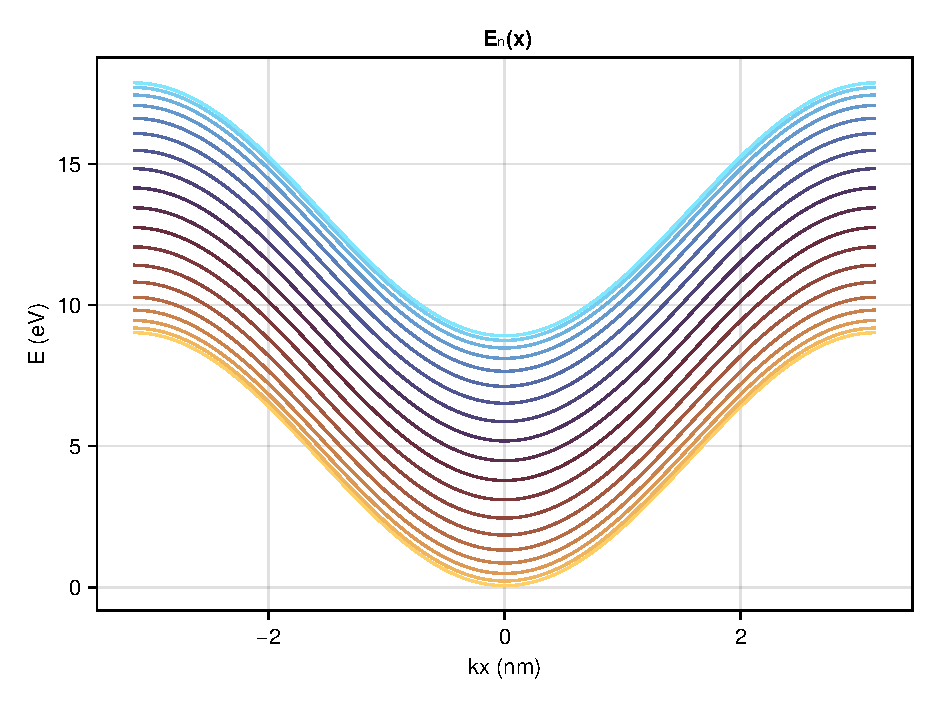
\includegraphics[width=0.7\linewidth]{ex1_disperssion_relation.pdf}
    \caption{Relacja dyspersji w jednorodnym kanale }
    \label{fig:ex1_dispersion_relation}
\end{figure}
%%%%%%%%%%%%%%%%%%%%%%%%%%%%%%%%%%%
Możemy zauważyć paraboliczny kształt relacji dyspersji dla \texttt{k\_x} bliskich zeru.
Dodatkowo, pierwsze energie charakteryzują się bliskimi siebie wartościami oraz tak samo końcowe - wartości środkowe są bardziej od siebie oddalone.
Nie zmienia to faktu, że każde z nich charakteryzują się tym samym kształtem.\\
\\
Ciągle pozostając w kanale wejściowym i wyjściowym przyjmując potencjał równy zeru, na układ spojrzymy inaczej - będziemy chcieli poznać \texttt{k\_x}.
Ponownie rozwiążemy równanie własne, jednak w tym przypadku uogólnione równanie własne
\begin{equation}
    \begin{bmatrix}
        0 & \mathbf{\hat{1}}\\
        \boldsymbol{\hat{\tau}} & E \mathbf{\hat{1}} - \mathbf{\hat{H}}
    \end{bmatrix}
    \begin{bmatrix}
        \mathbf{\hat{u}}\\
        \mathbf{\hat{w}}
    \end{bmatrix}
    -\lambda
    \begin{bmatrix}
        \mathbf{\hat{1}} & 0 \\
        0 & \boldsymbol{\hat{\tau}}^{\dagger}
    \end{bmatrix}
    \begin{bmatrix}
        \mathbf{\hat{u}}\\
        \mathbf{\hat{w}}
    \end{bmatrix}
    =
    0.
    \label{eq:uogolniony-problem-wlasny}
\end{equation}
W powyższym równaniu przyjęliśmy, że wektory $\boldsymbol{\psi}_{i-1}\equiv \mathbf{u}$ oraz $\boldsymbol{\psi}_i = \lambda \mathbf{u} \equiv \mathbf{w}$.
Wartość \texttt{k\_x} mieści się w wartościach własnych $\lambda$, które będą rozwiązywane.
Każda z macierzy będących elementami każdej z macierzy w uogólnionym problemie własnym ma wymiar \texttt{N\_y}, wobec tego uzyskujemy \texttt{2N\_y} wartości własnych $\lambda = \ee ^{\ii k_x ^{\pm}\Delta x}$ i wektorów własnych $\begin{bmatrix}
    \mathbf{u}_{\pm, n} & \boldsymbol{\lambda}_{\pm, n} & \mathbf{u}_{\pm, n}
\end{bmatrix}^T$.
Po rozwiązaniu równania postawiliśmy warunek \textit{segregujący} wektory i wartości $|\lambda_{\pm, n}| = 1$ uzyskując mody propagujące się.
Na ich podstawie można było wyznaczy prędkość i podzielić je na te propagujące w lewo i~prawo
\begin{equation}
    v_{\pm, n} = -\frac{2\Delta x}{\hbar}\mathfrak{Im}\left[\lambda_{\pm, n} \ \mathbf{u}^{\dagger}_{\pm, n}\boldsymbol{\tau}^{\dagger}\mathbf{u}_{\pm, n}\right].
\end{equation}
Z uzyskanych wartości własnych mogliśmy wyekstrahować wartości \texttt{k\_x = 1/(im * dx)log(lambda)}. 
W problemie~\eqref{eq:uogolniony-problem-wlasny} występuje wartość $E$ - będziemy zatem rozpatrywać wartości $E = \{0.2, 0.4\}~$eV.\\
\\
Wracając do relacji dyspersji na rysunku~\ref{fig:ex1_dispersion_relation} dla energii $E = 0.2$~eV powinniśmy zaobserwować 1 mod (dwa przecięcia $E = 0.2$~eV z relacją dyspersji) oraz dla $E = 0.4$~eV - dwa mody.
Na rysunku~\ref{fig:ex1e02} zostały przedstawione wyznaczone wartości \texttt{k\_x} dla każdego z przypadków ($E = 0.2$~eV: rys.~\ref{fig:ex1e02}, $E = 0.4$~eV: rys.~\ref{fig:ex1e04}).\\
%%%%%%%%%%%%%%%%%%%%%%%%%%%%%%%%%%%
%%%%%%%%%%%%%%%%%%%%%%%%%%%%%%%%%%%
\begin{figure}[htp!]
    \centering
\begin{subfigure}{.495\textwidth}
\centering
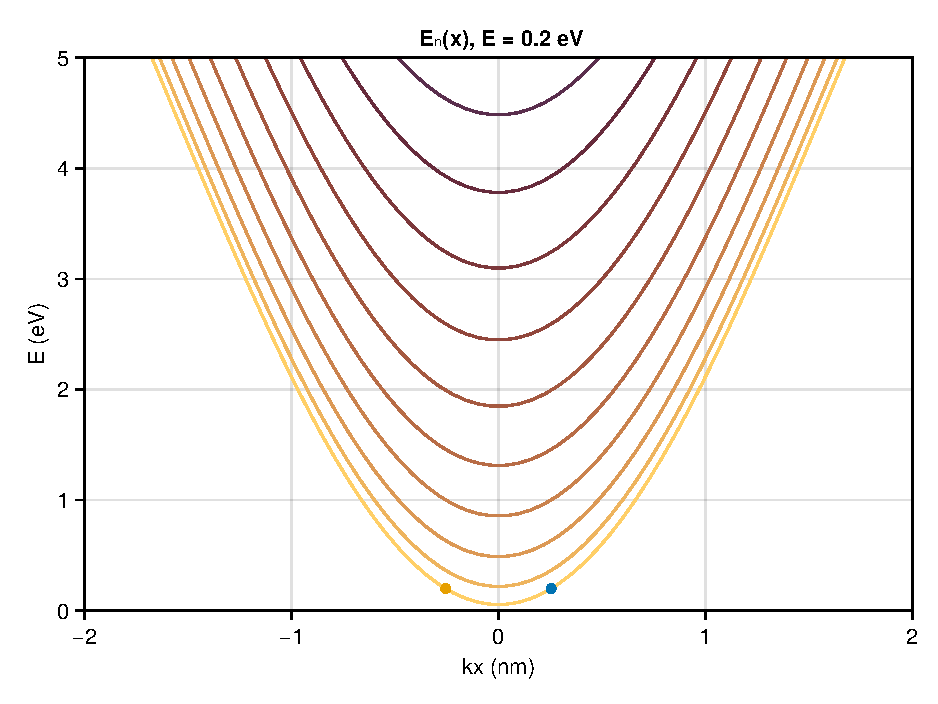
\includegraphics[width=1.0\textwidth]{ex2_disperssion_energy02.pdf}
    \caption{}
    \label{fig:ex1e02}
\end{subfigure}
\begin{subfigure}{.495\textwidth}
\centering
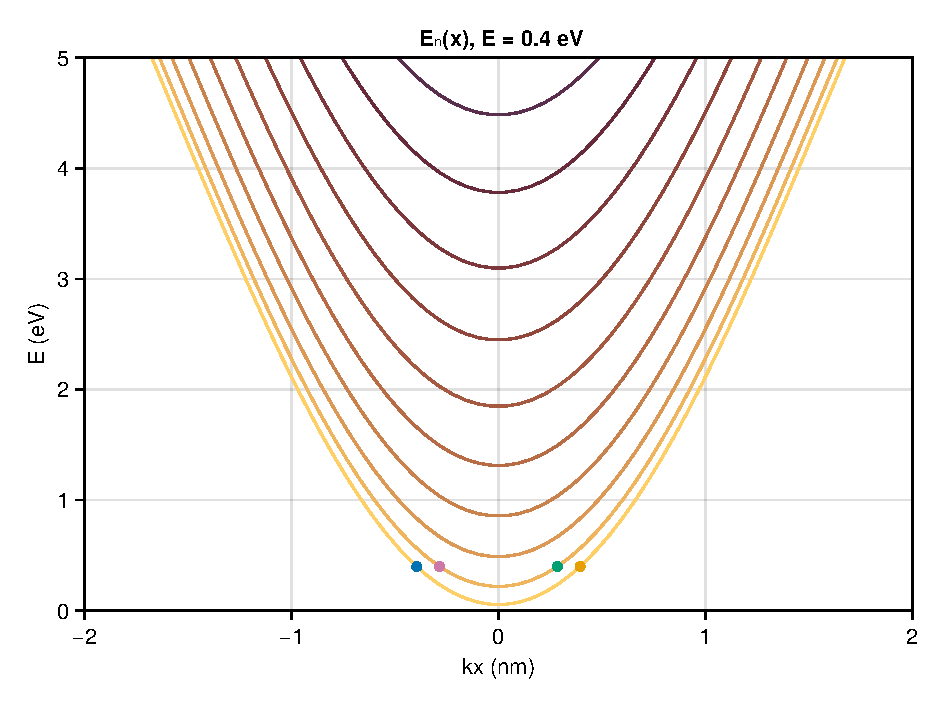
\includegraphics[width=1.0\textwidth]{ex2_disperssion_energy04.pdf}
    \caption{}
    \label{fig:ex1e04}
\end{subfigure}
\caption{Relacja dyspersji dla~\textbf{(a)}~$E = 0.2$~eV; \textbf{(b)}~$E =  0.4$~eV dla niższych energii.
Punkty reprezentują mody propagujące się w prawo i lewo}
\label{ex2_disp_rel_0204}
\end{figure}
%%%%%%%%%%%%%%%%%%%%%%%%%%%%%%%%%%%
\\
Korzystając ponownie z uzyskanych wektorów własnych możemy sprawdzić jak zachowują się części rzeczywiste i urojone (po normalizacji).
Oczywiście dla $E = 0.2~$eV uzyskaliśmy jedną wartość własną, której odpowiada jeden wektor własny, którego części zostały przedstawione na rysunku~\ref{fig:real_imag_02}.
Przy $E = 0.4$~eV uzyskaliśmy dwa wektory, co zostało przedstawione na rysunku~\ref{fig:real_imag_04}.
%%%%%%%%%%%%%%%%%%%%%%%%%%%%%%%%%%%
\begin{figure}[htp!]
    \centering
\begin{subfigure}{.495\textwidth}
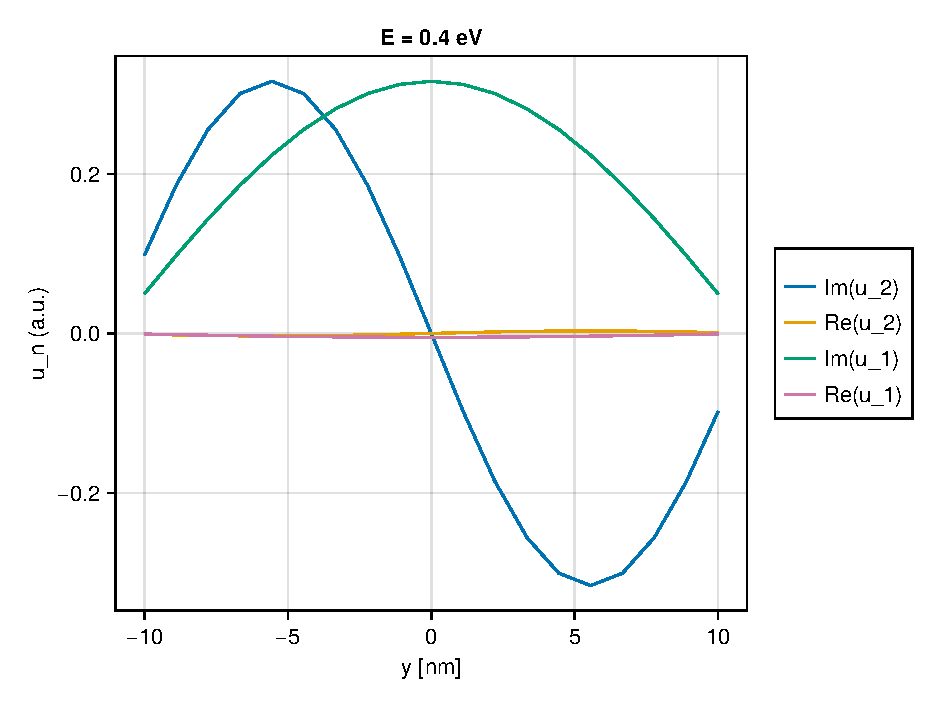
\includegraphics[width=1.0\textwidth]{ex2_imag_real_energy04.pdf}
    \caption{}
    \label{fig:real_imag_04}
\end{subfigure}
\begin{subfigure}{.495\textwidth}
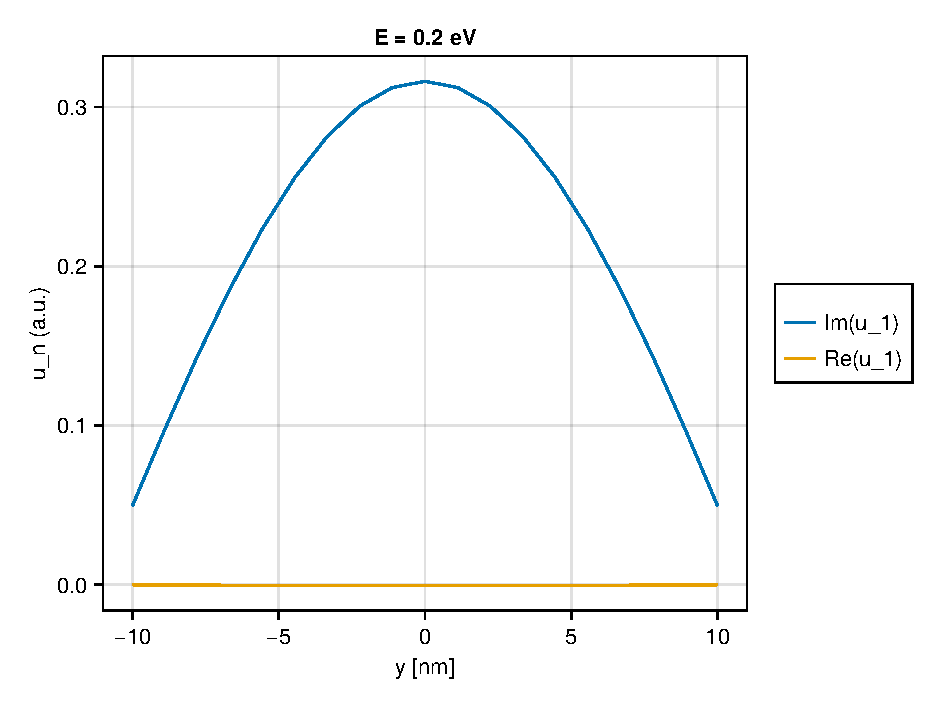
\includegraphics[width=1.0\textwidth]{ex2_imag_real_values_energy02.pdf}
    \caption{}
    \label{fig:real_imag_02}
\end{subfigure}
\caption{Część rzeczywista i urojona funkcji własnych $u_{-, n}$ dla~\textbf{(a)}~$E = 0.2$~eV; \textbf{(b)}~$E = 0.4$~eV}
\label{fig:ex2_real_imag0204}
\end{figure}
%%%%%%%%%%%%%%%%%%%%%%%%%%%%%%%%%%%
W pierwszym przypadku, możemy zauważyć podobne zachowanie, kształt krzywej dla części rzeczywistej i urojonej.
Jednak przy $E = 0.4~$eV obserwujemy dodatkowo sinusoidalny (określony na prawie całym okresie) kształt przy pierwszym stanie.
%%%%%%%%%%%%%%%%%%%%%%%%%%%%%%%%%%%
\section{Podsumowanie}
%%%%%%%%%%%%%%%%%%%%%%%%%%%%%%%%%%%
W ramach projektu wyznaczono relację dyspersji w jednorodnym kanale oraz obliczono propagujące mody dla wybranych energii, korzystając z rozwiązań uogólnionego problemu własnego. 
Przedstawiono zależność $E_k$, obliczono prędkości modów oraz zilustrowano ich profile.
Pozostała część projektu, dotycząca pełnej implementacji układu 2D i obliczeń $T/R$, nie została zrealizowana ze względu na trudności implementacyjne i brak uzyskania poprawnych wyników.
\end{document}
